\documentclass[tikz]{standalone}
\usetikzlibrary{arrows.meta}
\begin{document}

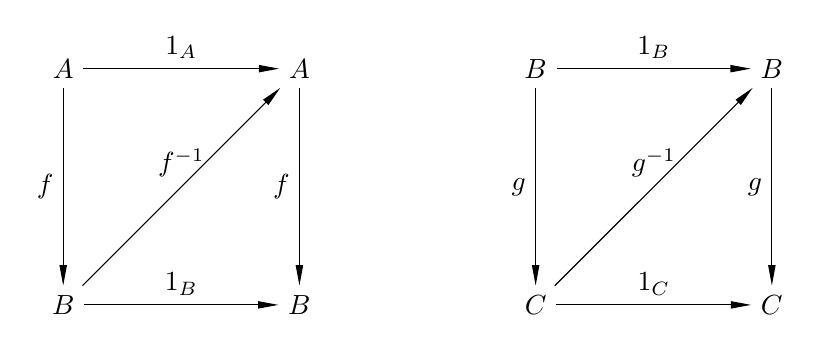
\begin{tikzpicture}[-latex, arrows={-Triangle[angle=20:5pt,scale=1.5]}]
	\node (A1) at (0,0) {\(A\)};
	\node (A2) at (3,0) {\(A\)};
	\node (B1) at (0,-3) {\(B\)};
	\node (B2) at (3,-3) {\(B\)};

	\draw (A1) to node [left] {\(f\)} (B1);
	\draw (A2) to node [left] {\(f\)} (B2);
	\draw (B1) to node [above] {\(f ^ {-1}\)} (A2);

	\draw (A1) to node [above] {\(1_A\)} (A2);
	\draw (B1) to node [above] {\(1_B\)} (B2);
	\begin{scope}[xshift=6cm]
		\node (B1) at (0,0) {\(B\)};
		\node (B2) at (3,0) {\(B\)};
		\node (C1) at (0,-3) {\(C\)};
		\node (C2) at (3,-3) {\(C\)};

		\draw (B1) to node [left] {\(g\)} (C1);
		\draw (B2) to node [left] {\(g\)} (C2);
		\draw (C1) to node [above] {\(g ^ {-1}\)} (B2);

		\draw (B1) to node [above] {\(1_B\)} (B2);
		\draw (C1) to node [above] {\(1_C\)} (C2);
	\end{scope}
\end{tikzpicture}

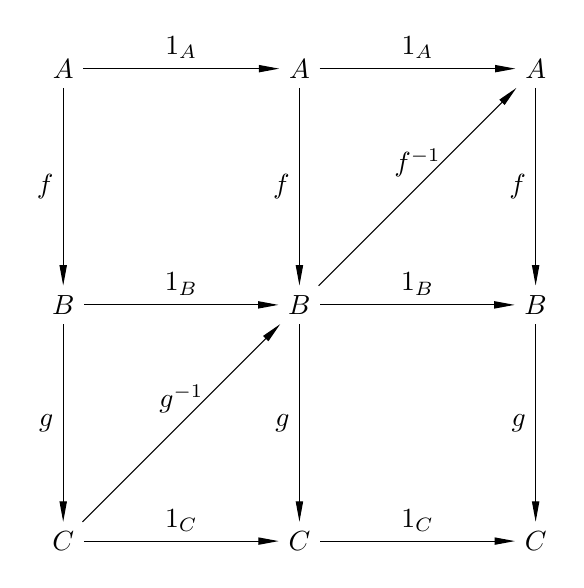
\begin{tikzpicture}[-latex, arrows={-Triangle[angle=20:5pt,scale=1.5]}]
	\node (A0) at (-3,0) {\(A\)};
	\node (A1) at (0,0) {\(A\)};
	\node (A2) at (3,0) {\(A\)};

	\node (B0) at (-3,-3) {\(B\)};
	\node (B1) at (0,-3) {\(B\)};
	\node (B2) at (3,-3) {\(B\)};

	\node (C0) at (-3,-6) {\(C\)};
	\node (C1) at (0,-6) {\(C\)};
	\node (C2) at (3,-6) {\(C\)};

	\draw (A0) to node [left] {\(f\)} (B0);
	\draw (A1) to node [left] {\(f\)} (B1);
	\draw (A2) to node [left] {\(f\)} (B2);
	\draw (B1) to node [above] {\(f ^ {-1}\)} (A2);

	\draw (B0) to node [left] {\(g\)} (C0);
	\draw (B1) to node [left] {\(g\)} (C1);
	\draw (B2) to node [left] {\(g\)} (C2);
	\draw (C0) to node [above] {\(g ^ {-1}\)} (B1);

	\draw (A0) to node [above] {\(1_A\)} (A1);
	\draw (A1) to node [above] {\(1_A\)} (A2);
	\draw (B0) to node [above] {\(1_B\)} (B1);
	\draw (B1) to node [above] {\(1_B\)} (B2);
	\draw (C0) to node [above] {\(1_C\)} (C1);
	\draw (C1) to node [above] {\(1_C\)} (C2);

\end{tikzpicture}

\end{document}
